\usepackage{graphicx,comment,framed}
\usepackage{amsthm,amssymb,amsmath}
\usepackage[rgb]{xcolor}
\usepackage{amssymb,amsmath}
\usepackage[colorlinks,linkcolor=blue,citecolor=blue]{hyperref}\usepackage{amsmath}
\usepackage{amsfonts}
\usepackage{amssymb}
\usepackage[usenames,dvipsnames]{pstricks}
\usepackage{graphicx,subfigure,wrapfig, relsize}
\usepackage{geometry,fancyhdr}
\usepackage[mathscr]{euscript}
\usepackage{multicol}
\usepackage{setspace}
\usepackage{tikz}
\usepackage{tabularx}
\usepackage{algorithmicx,algorithm}
\usepackage{mdframed}
\usepackage[noend]{algpseudocode}


%------------------------ Algorithm ------------------------------------

%\newenvironment{الگوریتم}[1]
%	{\bigskip\bigskip\begin{algorithm}\caption{#1} \label{الگوریتم: #1}\vspace{0.5em}\begin{algorithmic}[1]}
%	{\end{algorithmic}\vspace{0.5em}\end{algorithm}\bigskip}
	

%\renewcommand{\algorithmicfor}{{به ازای}}
%\renewcommand{\algorithmicwhile}{{تا وقتی}}
%\renewcommand{\algorithmicdo}{\hspace{-.2em}:}
%\renewcommand{\algorithmicif}{{اگر}}
%\renewcommand{\algorithmicthen}{\hspace{-.2em}:}
%\renewcommand{\algorithmicelse}{{در غیر این صورت:}}
%\renewcommand{\algorithmicelsif}{{در غیر این صورت اگر: }}
%\renewcommand{\algorithmicreturn}{{برگردان}}
%\renewcommand{\algorithmiccomment}[1]{$\triangleleft$ \emph{#1}}
%\renewcommand{\algorithmicrequire}{\textbf{ورودی:}}
%\renewcommand{\algorithmicensure}{\textbf{خروجی:}}

%\newcommand{\اگر}{\If}
%\newcommand{\وگرنه}{\Else}
%\newcommand{\وگر}{\ElsIf}
%\newcommand{\پایان‌اگر}{\EndIf}
%\newcommand{\به‌ازای}{\For}
%\newcommand{\پایان‌به‌ازای}{\EndFor}
%\newcommand{\تاوقتی}{\While}
%\newcommand{\پایان‌تاوقتی}{\EndWhile}
%\newcommand{\دستور}{\State}
%\newcommand{\دستورک}{\Statex}
%\newcommand{\توضیحات}{\Comment}
%\newcommand{\برگردان}{\Return}
%\renewcommand{\ورودی}{\Require}
%\newcommand{\خروجی}{\Ensure}

\usepackage{fontspec}
\usepackage{xepersian}
\usepackage{physics}


%--------------------- page settings ----------------------

\settextfont[Scale = 1 ,
             BoldFont = *Bd ,
			 ItalicFont = *It ,
			 BoldItalicFont = *BdIt ,
             Extension = .ttf]{XB Niloofar}

\setdigitfont[Scale = 0.9 ,
             BoldFont = *Bd ,
			 ItalicFont = *It ,
			 BoldItalicFont = *BdIt ,
             Extension = .ttf]{XB Niloofar}

\setlatintextfont[Scale=1.1]{Times New Roman}

\defpersianfont\sayeh[Scale=1.2]{XB KayhanPook.ttf}

\addtolength{\textheight}{3.8cm}
\addtolength{\topmargin}{-22mm}
\addtolength{\textwidth}{2.7cm}
\addtolength{\oddsidemargin}{-1.5cm}


%------------------------ Environments ------------------------------------

\newtheorem{قضیه}{قضیه}
\newtheorem{لم}{لم}
\newtheorem{مشاهده}{مشاهده}
\newtheorem{تعریف}{تعریف}


%-------------------------- Notations ------------------------------------

\newcommand{\IR}{\ensuremath{\mathbb{R}}} 
\newcommand{\IZ}{\ensuremath{\mathbb{Z}}} 
\newcommand{\IN}{\ensuremath{\mathbb{N}}} 
\newcommand{\IS}{\ensuremath{\mathbb{S}}} 
\newcommand{\IC}{\ensuremath{\mathbb{C}}} 
\newcommand{\IB}{\ensuremath{\mathbb{B}}} 

\newcommand{\bR}{\mathbb{R}}
\newcommand{\cB}{\mathcal{B}}
\newcommand{\cO}{\mathcal{O}}
\newcommand{\cG}{\mathcal{G}}
\newcommand{\rM}{\mathrm{M}}
\newcommand{\rC}{\mathrm{C}}
\newcommand{\rV}{\mathrm{V}}

\newcommand{\lee}{\leqslant}
\newcommand{\gee}{\geqslant}
\newcommand{\ceil}[1]{{\left\lceil{#1}\right\rceil}}
\newcommand{\floor}[1]{{\left\lfloor{#1}\right\rfloor}}
\newcommand{\prob}[1]{{\mbox{\tt Pr}[#1]}}
\newcommand{\set}[1]{{\{ #1 \}}}
\newcommand{\seq}[1]{{\left< #1 \right>}}
\newcommand{\provided}{\,|\,}
\newcommand{\poly}{\mbox{\rm poly}}
\newcommand{\polylog}{\mbox{\rm \scriptsize polylog}\,}
\newcommand{\comb}[2] {\left(\!\!\begin{array}{c}{#1}\\{#2}\end{array}\!\!\right)}

\newcommand{\REM}[1]{}
\newcommand{\mrbox}[1]{\mbox{\lr{#1}}}


\newcounter{probcnt}
\newcommand{\مسئله}[1]{\stepcounter{probcnt}\bigskip\bigskip{
 	\large \bf پاسخ مسئله‌ی \arabic{probcnt}$\mbox{\bf{.}}$ \ #1} \bigskip}

\newcommand{\fqed}[1]{\leavevmode\unskip\nobreak\quad\hspace*{\fill}{\ensuremath{#1}}}

\newenvironment{اثبات}
	{\begin{trivlist}\item[\hskip\labelsep{\em اثبات.}]}
	{\fqed{\square}\end{trivlist}}

\newenvironment{حل}
	{\begin{trivlist}\item[\hskip\labelsep{\bf حل.}]}
	{\fqed{\blacktriangleright}\end{trivlist}}

\ifdefined\hidesols
	\newsavebox{\trashcan} % uncomment the following line to hide solutions
	\renewenvironment{حل}{\begin{latin}\begin{lrbox}{\trashcan}}{\end{lrbox}\end{latin}}
\fi


%------------------------- Header -----------------------------

\newcommand{\سربرگ}[3]{
\parindent=0em

\rightline{
\makebox[6em][c]{
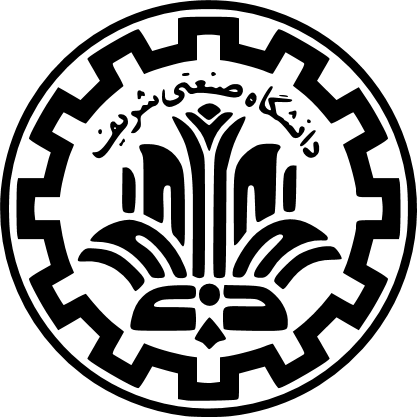
\includegraphics[height=1.6cm]{../commons/sharif.png}
}}
\vspace{-.2em}
{\scriptsize\bf دانشکده‌ی مهندسی کامپیوتر}
\hfill {\small
شایان صالحی \ 
}\\[-6em]
\leftline{\hfill\Large\bf 
سیگنال‌ها و سیستم‌ها
}\\[.7em]
\leftline{\hfill\bf 
نیم‌سال دوم ۰۴-۰۵
}\\[0.7em]
\hrule height .12em
\vspace{-2mm}
\normalsize
\vspace{1mm} #1
\hfill \small  #3
\vspace{1mm} 
\hrule height .1em

\vspace{-2.7em} 
\hfill {\sayeh\large #2} \hfill
}

% ------------------------------ Sample Input/Output --------------------------


% Bases on: https://github.com/admp/LIO-LaTeX/tree/master/other/neerc-acm

\def\s@tm@cr@s{%
\def\widthin##1{\exmpwidinf=##1\relax}\def\widthout##1{\exmpwidouf=##1\relax}%
\def\stretchin##1{\advance\exmpwidinf by ##1\relax}%
\def\stretchout##1{\advance\exmpwidouf by ##1\relax}%
}%

\newenvironment{example*}[3][]{%
\s@tm@cr@s\ttfamily\obeylines\obeyspaces\frenchspacing%\testst@r#1%
\newcommand{\exmp}[2]{%
\begin{minipage}[t]{#2}\rightskip=0pt plus 1fill\relax##1\medskip\end{minipage}&%
\begin{minipage}[t]{#3}\rightskip=0pt plus 1fill\relax##2\medskip\end{minipage}\\%
\hline}%
\begin{tabular}{|l|l|}
\hline
\multicolumn{1}{|c|}{\bf\rl{ورودی نمونه}}&%
\multicolumn{1}{|c|}{\bf\rl{خروجی نمونه}}\\%
\hline
}
{\end{tabular}}

\newenvironment{example}
	{\begin{example*}{.47\textwidth}{.475\textwidth}}
	{\end{example*}}

% ------------------------------ Table Settings --------------------------

\newcolumntype{Y}{>{\centering\arraybackslash}X}

\definecolor{lightgreen}{rgb}{0.95, 0.99, 0.97}

\newmdenv[
	topline=false,
	bottomline=false,
	skipabove=\topsep,
	skipbelow=\topsep,
	backgroundcolor=lightgreen,
	innerleftmargin=10pt,
	innerrightmargin=10pt,
	innertopmargin=10pt,
	innerbottommargin=10pt,
	leftmargin=10pt,
	rightmargin=10pt,
	leftline=false,
	rightline=false,
	linewidth=1pt
]{siderules}
	
\newenvironment{examplebox}[0]
	{\begin{siderules}\par\nobreak}
	{\end{siderules}}
	  

\newcolumntype{M}{>{$}c<{$}}